\documentclass[12pt,a4paper]{article}
\usepackage[utf8]{inputenc}
\usepackage[T1]{fontenc}
\usepackage{lmodern}
\usepackage{amsmath,amssymb}
\usepackage{siunitx}
\usepackage{geometry}
\usepackage{hyperref}
\usepackage{enumitem}
\usepackage{tikz}
\geometry{margin=2.2cm}

\title{Lecture 2 -- Feedback, Non-Ideal Op-Amp Gain and Impedances}
\author{Readable Assignment Set}
\date{}

\begin{document}
\maketitle
\tableofcontents

\section{Assignments}
\subsection{B1}
For the shown circuit (with $R_1=\SI{1.0}{M\Omega}$, $R_2=\SI{1.0}{M\Omega}$, $R_3=\SI{10.2}{k\Omega}$, $R_4=\SI{1.0}{M\Omega}$):
\begin{enumerate}
\item Find symbolic and numerical values for $\alpha$.
\item Find symbolic and numerical values for $\beta$.
\item Find symbolic and numerical values for $A_{SIGN}=v_o/v_{in}$.
\item Explain an advantage of this circuit compared with a standard inverting amplifier.
\end{enumerate}
Then replace the ideal op-amp by a \(\mu\)A741C at \SI{25}{\celsius}, supplies \(\pm\SI{15}{V}\):
\begin{enumerate}[resume]
\item Find the maximum percentage error in $A_{SIGN}$ from finite open-loop gain.
\item Compute a typical value for $Z_o$.
\item Compute the minimum value for $Z_{in}$.
\end{enumerate}

\subsection{B2}
Investigate non-ideal effects (finite $A_{OL}$, finite $R_{in}$, nonzero $R_o$) for a voltage follower:
\begin{enumerate}[label=\alph*)]
\item Derive $v_o/v_s$, evaluate for $A_{OL}=10^5$, $R_{in}=\SI{1}{M\Omega}$, $R_o=\SI{25}{\Omega}$, compare with ideal.
\item Derive $Z_{in}=v_s/i_s$, evaluate numerically, compare with ideal.
\item Derive output impedance $Z_o$, evaluate numerically, compare with ideal.
\end{enumerate}

\section{Hints}
\subsection{B1}
\begin{itemize}
\item Express the closed-loop gain as $A_{CL}=\dfrac{\alpha A_{OL}}{1+\beta A_{OL}}=\dfrac{\alpha}{\beta}\cdot K_f$ where $K_f=\dfrac{\beta A_{OL}}{1+\beta A_{OL}}$.
\item For large loop gain ($\beta A_{OL}\gg 1$), $A_{CL}\approx \alpha/\beta$.
\item Percentage gain error from finite $A_{OL}$ is approximately $\dfrac{1}{\beta A_{OL}}\cdot100\%$.
\item Closed-loop output impedance is reduced by feedback approximately as $Z_{o,cl}\approx Z_{o,ol}/(1+\beta A_{OL})$.
\end{itemize}

\subsection{B2}
\begin{itemize}
\item Use the op-amp equation $v_o=A_{OL}(v_+-v_-)$ with follower relation $v_+=v_s$, $v_-=v_o$ (including loading where needed).
\item Keep source current as sum of op-amp input current and any current forced by finite output/input interactions.
\item For follower output impedance, inject a test current at output with source set to zero.
\end{itemize}

\section{Step-by-step solutions}
\subsection{B1}
\begin{enumerate}
\item Write node equations to identify feedforward coefficient $\alpha$ and feedback coefficient $\beta$ from the given resistor network.
\item Compute ideal gain as $A_{ideal}=\alpha/\beta$.
\item Closed-loop with finite open-loop gain: 
\[
A_{SIGN}=\frac{\alpha A_{OL}}{1+\beta A_{OL}}.
\]
\item Advantage versus simple inverting stage: much higher effective input resistance at the source while preserving a controlled gain (depends on exact topology).
\item Maximum percentage gain error:
\[
\varepsilon_{A,\%}=\left|\frac{A_{ideal}-A_{SIGN}}{A_{ideal}}\right|\cdot100\%
=\frac{1}{1+\beta A_{OL}}\cdot100\% \approx \frac{100\%}{\beta A_{OL}}.
\]
\item Typical closed-loop output impedance:
\[
Z_o\approx \frac{R_{o,741}}{1+\beta A_{OL}}.
\]
Use typical \(\mu\)A741C data for $R_{o,741}$ and $A_{OL}$.
\item Minimum input impedance: include finite op-amp differential input resistance reflected by feedback and the external resistor network as seen by $v_{in}$.
\end{enumerate}

\subsection{B2(a) Voltage gain}
For a voltage follower with non-ideal op-amp model, first-order gain:
\[
\frac{v_o}{v_s}\approx\frac{A_{OL}}{1+A_{OL}}\cdot\frac{R_L}{R_L+R_o}
\]
(if load $R_L$ is present explicitly). For large $R_L$ this becomes $A_{OL}/(1+A_{OL})$.
With $A_{OL}=10^5$, ideal result is 1, practical result is very close to 1.

\subsection{B2(b) Input impedance}
\[
Z_{in,cl}\approx R_{in}(1+A_{OL})
\]
for the follower model (dominant effect of bootstrapping). With $R_{in}=\SI{1}{M\Omega}$ and $A_{OL}=10^5$, this is extremely high and far above the idealized finite-network case.

\subsection{B2(c) Output impedance}
\[
Z_{o,cl}\approx \frac{R_o}{1+A_{OL}}=\frac{25}{100001}\,\Omega\approx\SI{0.25}{m\Omega}.
\]
Thus practical $Z_o$ is tiny and close to ideal zero.

\subsection{Conceptual feedback sketch}
\begin{center}
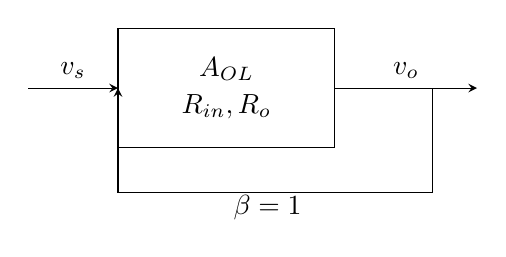
\begin{tikzpicture}[scale=0.95,>=stealth]
\draw[->] (-3,0) -- (-1.8,0) node[midway,above] {$v_s$};
\draw (-1.8,-0.8) rectangle (1.1,0.8);
\node at (-0.35,0.25) {$A_{OL}$};
\node at (-0.35,-0.25) {$R_{in},R_o$};
\draw[->] (1.1,0) -- (3,0) node[midway,above] {$v_o$};
\draw[->] (2.4,0) |- (0,-1.4) -| (-1.8,0);
\node at (0.2,-1.6) {$\beta=1$};
\end{tikzpicture}
\end{center}

\end{document}
